\documentclass[border=5]{standalone}
\usepackage{tikz}
\usepackage{csvsimple}
\usepackage{xfp}

\newcommand*{\xMin}{0}%
\newcommand*{\xMax}{2.5}%
\newcommand*{\yMin}{0}%
\newcommand*{\yMax}{2.5}%
\begin{document}

  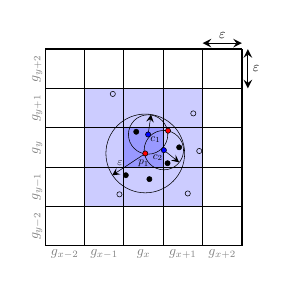
\begin{tikzpicture}
    \draw[fill=blue!20] (0.50, 0.50) rectangle (2.00, 2.00);
    \draw[fill=blue!40] (1.00, 1.00) rectangle (1.50, 1.50);
    \draw[step=0.5, black, thin] (0, 0) grid (2.5, 2.5);
    
    \node [gray,scale=0.5]  at (0.25,-0.1) {$g_{x-2}$};
    \node [gray,scale=0.5]  at (0.75,-0.1) {$g_{x-1}$};
    \node [gray,scale=0.5]  at (1.25,-0.1) {$g_{x}$};
    \node [gray,scale=0.5]  at (1.75,-0.1) {$g_{x+1}$};
    \node [gray,scale=0.5]  at (2.25,-0.1) {$g_{x+2}$};

    \node [gray,scale=0.5,rotate=90]  at (-0.1,0.25) {$g_{y-2}$};
    \node [gray,scale=0.5,rotate=90]  at (-0.1,0.75) {$g_{y-1}$};
    \node [gray,scale=0.5,rotate=90]  at (-0.1,1.25) {$g_{y}$};
    \node [gray,scale=0.5,rotate=90]  at (-0.1,1.75) {$g_{y+1}$};
    \node [gray,scale=0.5,rotate=90]  at (-0.1,2.25) {$g_{y+2}$};
    
    \coordinate (P1) at (1.272, 1.174); 
    \coordinate (P2) at (1.561, 1.463);
    \coordinate (C1) at (1.308, 1.415);
    \coordinate (C2) at (1.508, 1.216);

    \draw[very thin] (C1) circle (0.25);
    \draw[very thin] (C2) circle (0.25);
    \draw[very thin] (P1) circle (0.50);
    
    \draw[-stealth, very thin] (P1) -- (0.8511, 0.896); 
    \draw[-stealth, very thin] (C1) -- (1.3455, 1.668);
    \draw[-stealth, very thin] (C2) -- (1.7022, 1.061);

    \node[draw, very thin, circle, scale=0.2, fill=red]  at (P1) {};
    \node[draw, very thin, circle, scale=0.2, fill=red]  at (P2) {};
    \node[draw, very thin, circle, scale=0.2, fill=blue] at (C1) {};
    \node[draw, very thin, circle, scale=0.2, fill=blue] at (C2) {};
    
    \node[draw, very thin, circle, scale=0.2, fill] at (1.157, 1.449) {};
    \node[draw, very thin, circle, scale=0.2, fill] at (1.025, 0.898) {};
    \node[draw, very thin, circle, scale=0.2, fill] at (1.555, 1.050) {};
    \node[draw, very thin, circle, scale=0.2, fill] at (1.324, 0.848) {};
    \node[draw, very thin, circle, scale=0.2, fill] at (1.702, 1.252) {};
    
    \node[draw, very thin, circle, scale=0.2] at (0.8595505617977528, 1.9297752808988764) {};
    \node[draw, very thin, circle, scale=0.2] at (0.9438202247191011, 0.6544943820224719) {};
    \node[draw, very thin, circle, scale=0.2] at (1.8117977528089888, 0.6657303370786517) {};
    \node[draw, very thin, circle, scale=0.2] at (1.9578651685393258, 1.2050561797752808) {};
    \node[draw, very thin, circle, scale=0.2] at (1.8820224719101124, 1.6825842696629214) {};
    
    \node[scale=0.4] at (1.25, 1.05) {$p_1$};
    \node[scale=0.4] at (1.40, 1.35) {$c_1$};
    \node[scale=0.4] at (1.43, 1.12) {$c_2$};
    \node[scale=0.4] at (0.95, 1.05) {$\varepsilon$};
    \draw[stealth-stealth] (\xMax - 0.5, \yMax + 0.075) -- (\xMax, \yMax + 0.075) node[midway, above, scale=0.5] {$\varepsilon$};
    \draw[stealth-stealth] (\xMax + 0.075, \yMax - 0.5) -- (\xMax + 0.075, \yMax) node[midway, right  , scale=0.5] {$\varepsilon$};
    

  \end{tikzpicture}

\end{document}
